\documentclass{standalone}
\usepackage{tikz}
\usetikzlibrary{shapes.geometric}

\begin{document}

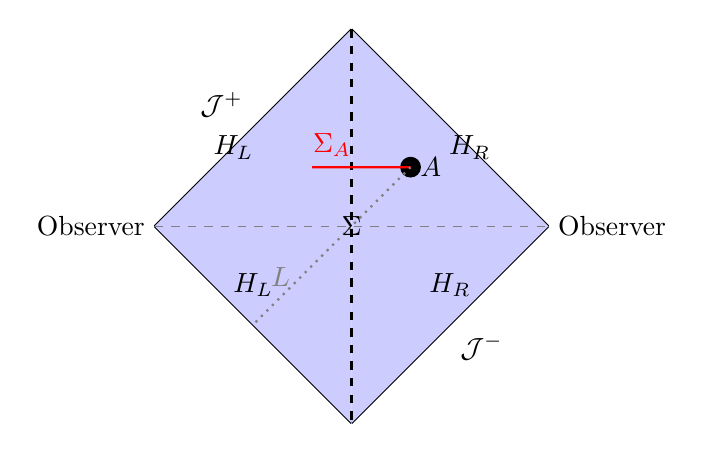
\begin{tikzpicture}[scale=2.5]

% Define coordinates for the vertices of the diamond
\coordinate (J+) at (0, 1);
\coordinate (J-) at (0, -1);
\coordinate (L) at (-1, 0);
\coordinate (R) at (1, 0);

% Draw the diamond
\draw[thick] (J+) -- (L) node[midway, above left] {$\mathcal{J}^+$};
\draw[thick] (J+) -- (R);
\draw[thick] (J-) -- (L);
\draw[thick] (J-) -- (R) node[midway, below right] {$\mathcal{J}^-$};

% Fill the static patches (blue regions)
\fill[blue!20] (J+) -- (L) -- (J-) -- cycle;
\fill[blue!20] (J+) -- (R) -- (J-) -- cycle;

% Draw the cosmological horizons H_L and H_R
\draw[dashed, very thick] (J+) -- (J-);
\node at (-0.6, 0.4) {$\text{H}_\text{L}$};
\node at (0.6, 0.4) {$\text{H}_\text{R}$};

% Draw the global spacelike slice (dashed line)
\draw[dashed, gray] (L) -- (R);

% Place the point A and label it
\coordinate (A) at (0.3, 0.3);
\fill[black] (A) circle (1.5pt) node[right] {$A$};

% Draw the red segment \Sigma_A
\draw[red, thick] (-0.2, 0.3) -- (A) node[midway, above left] {$\Sigma_A$};

% Draw the future light sheet emanating from A (dotted line)
\draw[dotted, gray, thick] (A) -- ++(-0.8, -0.8) node[pos=0.7, left] {$L$};

% Add labels for the observers
\node[left] at (L) {Observer};
\node[right] at (R) {Observer};

% Add labels for the static patches P_L and P_R
\node at (-0.5, -0.3) {$\text{H}_\text{L}$};
\node at (0.5, -0.3) {$\text{H}_\text{R}$};

% Add the label for the global spacelike slice
\node at (0, 0) {$\Sigma$};

\end{tikzpicture}

\end{document}